\section{Simulation Analysis }
\label{sec:simulation}

\subsection{Operating Point Analysis for $t<0$}

Table~\ref{tab:SIM_PASSO1} shows the simulated operating point results for the circuit under analysis for $t<0$.
%Colocar a tabela 
\begin{table}[h]
  \centering
  \begin{tabular}{|l|r|}
    \hline    
    {\bf Name} & {\bf Value [A or V]} \\ \hline
    \input{../sim/PASSO1_tab}
  \end{tabular}
  \caption{Operating point for $t<0$. A variable preceded by @ is of type {\em current}
    and expressed in Ampere; other variables are of type {\it voltage} and expressed in
    Volt.}
  \label{tab:SIM_PASSO1}
\end{table}

It is important to notice that it has been necessary to implement an extra test voltage sorce  between the node 7 and $R_6$ providing 0V so that is does not interfere with the rest of the circuit and enable us to measure the voltage $V_d$ flowing in the dependent source. Therefore, this creation does not change any results and it is only based on the Ngspice requirements to define a current controlled voltage source.

Compared to the theoretical analysis the simulation showed practically identical results, except for a small divergence in the last decimal place that probably occurs when Ngspice rounds the numbers. Thus, the maximum relative error is $10^{-5}$. It is worth mentioning that Ngspice software also uses the same mathematical methods as octave to find results, hence, this result was already expected.


\subsection{Operating Point Analysis for $t=0$}

The circuit was simulated using an operating point analysis with $V_s(0)=0$ and replacing que capacitor with a voltage source $V_c=V(6)-V(8)$ as these were obtained in the previous step. This step in required to compute the boundary conditions that ensure the continuity in the capacitor. Table~\ref{tab:SIM_PASSO2} shows the results of the simulation. Notice that:  \begin{equation}
R_{eq}=\frac{V_{c}}{I_{c}}
\end{equation}

\begin{table}[h]
  \centering
  \begin{tabular}{|l|r|}
    \hline    
    {\bf Name} & {\bf Value [A or V]} \\ \hline
    \input{../sim/PASSO2_tab}
  \end{tabular}
  \caption{Operating point for $t=0$. A variable preceded by @ is of type {\em current}
    and expressed in Ampere; other variables are of type {\it voltage} and expressed in
    Volt.}
  \label{tab:SIM_PASSO2}
\end{table}

\subsection{Natural Solution for $V_6$}

In order to study the natural response of the circuit in the interval [0,20]ms, a transient analysis was made, using the results for $V_6$ and $V_8$ computed in the previous step. Figure \ref{fig:SIM_NAT_SOL} shows the results for the natural solution for $V_6$.

\begin{figure}[h] \centering
\vspace{-3cm}
\includegraphics[height=10cm]{../sim/trans.pdf}
\caption{Natural solution of $v_6(t)$.}
\label{fig:SIM_NAT_SOL}
\end{figure}

\newpage
\subsection{Total Solution for $V_6$}

The results obtained in the last section were used to make this analysis,but considering $V_s$ a sinusoidal voltage source with f=1kHz. The total response of the circuit is the result of summing the natural analysis with the forced one (natural + forced). 
Figure \ref{fig:SIM_TOT_SOL} shows the transient analysis results for $V_s(t)$.

\begin{figure}[h] \centering
\includegraphics[height=12cm]{../sim/trans2.pdf}
\caption{Natural solution of $v_6(t)$ and $V_s$.}
\label{fig:SIM_TOT_SOL}
\end{figure}

\newpage
\subsection{Frequency Response}


In this section, the frequency range considered to analyze the frequency response in node 6 is from 0.1 Hz to 1 MHz. The figures show the magnitude and phase of the frequency response for $V_s$, $V_c$ and $V_6$.

\begin{figure}[h] \centering
\vspace{-3cm}
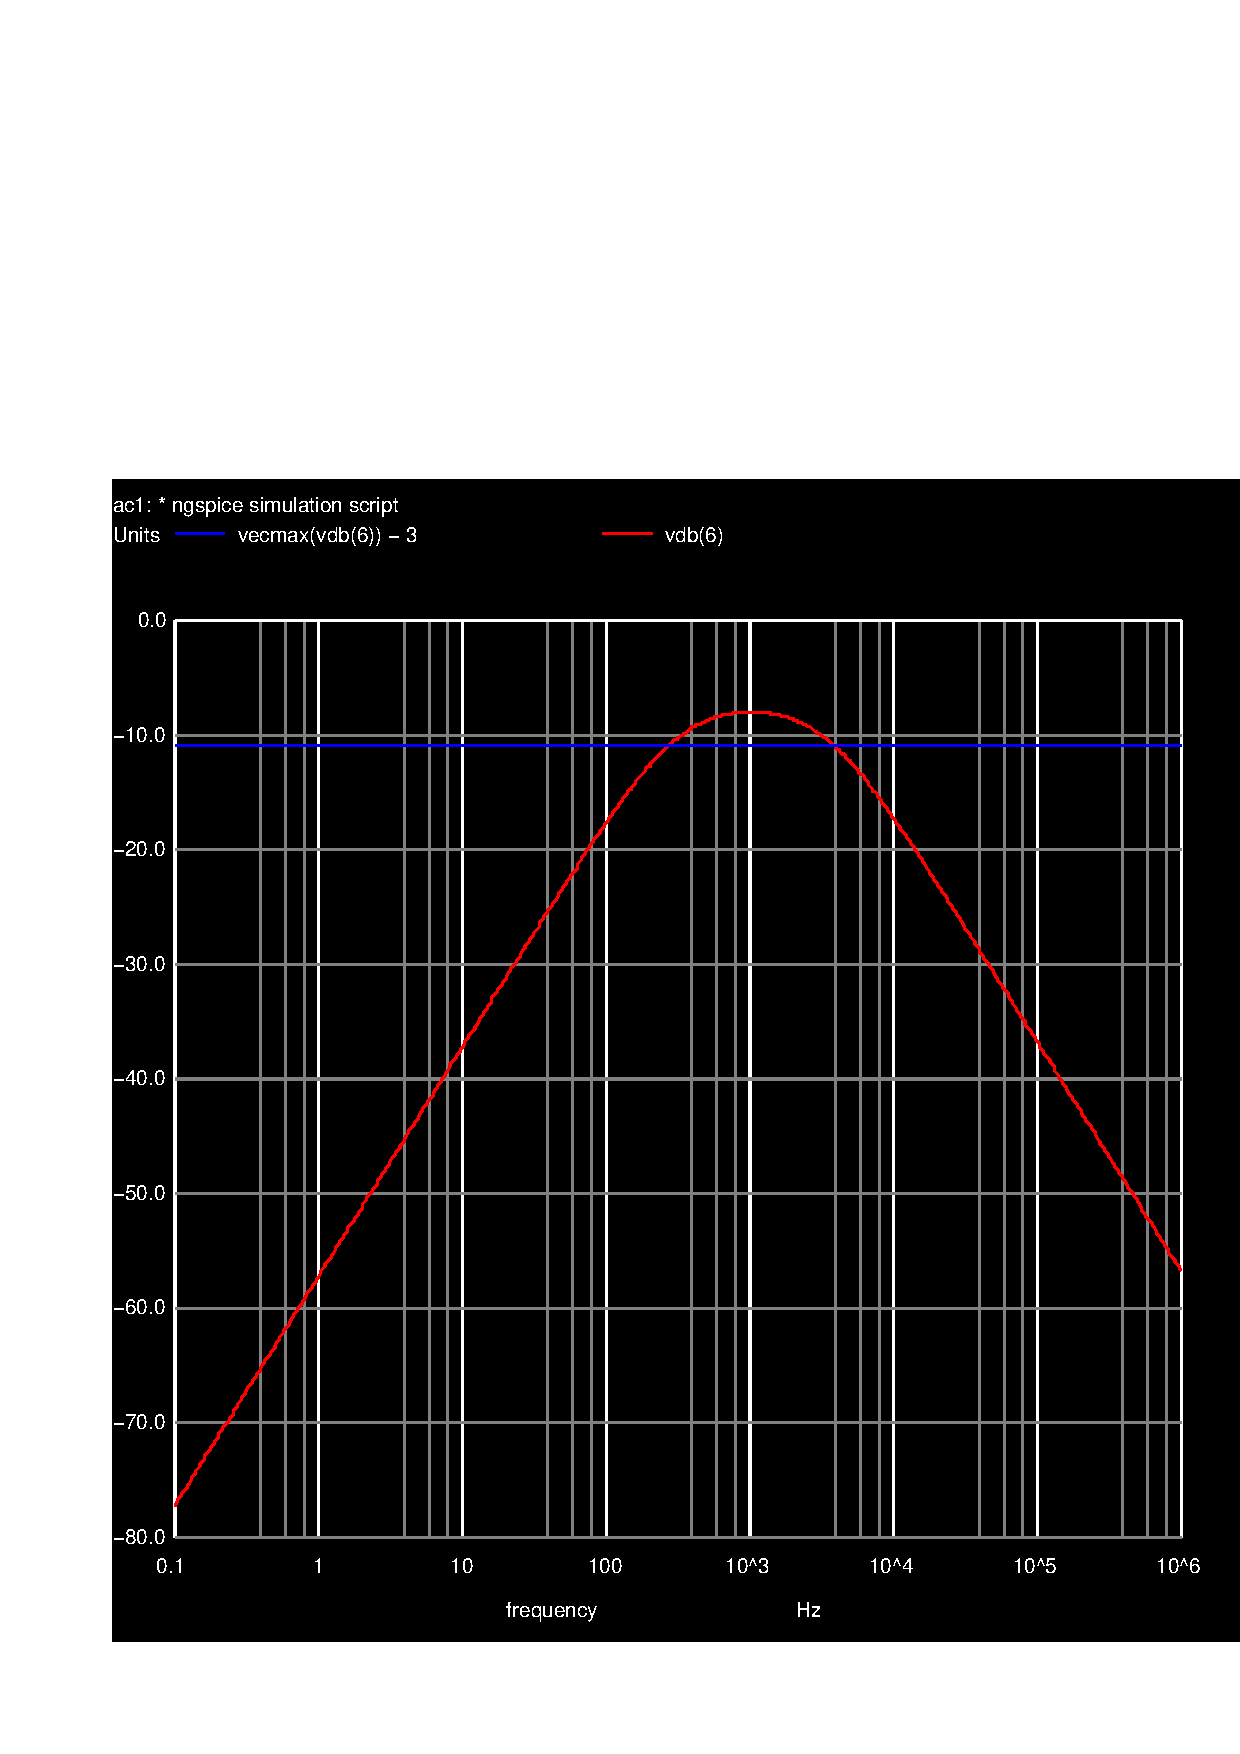
\includegraphics[height=10cm]{../sim/db.pdf}
\caption{Magnitude response of $V_s$, $v_6(t)$ and $V_c(t)$.}
\label{fig:SIM_MAG}
\end{figure}

\begin{figure}[h] \centering
\vspace{-3cm}
\includegraphics[height=10cm]{../sim/ph.pdf}
\caption{Angle response of $V_s$, $v_6(t)$ and $V_c(t)$.}
\label{fig:SIM_ANG}
\end{figure}

When comparing the graphics obtained in Ngspice and Octave, the similarity between the results is noticeable and small differences can be explained by approximation errors.



